\item[\textbf{5.}] \textbf{[15 min/10 puntos]} \textcolor{dkgreen}{En una píla asíncrona, el hilo $p$ termina su operación y el sistema entra en un periodo de ``inactividad''.}
\begin{figure}[H]
    \centering
    \vspace{-10pt}
    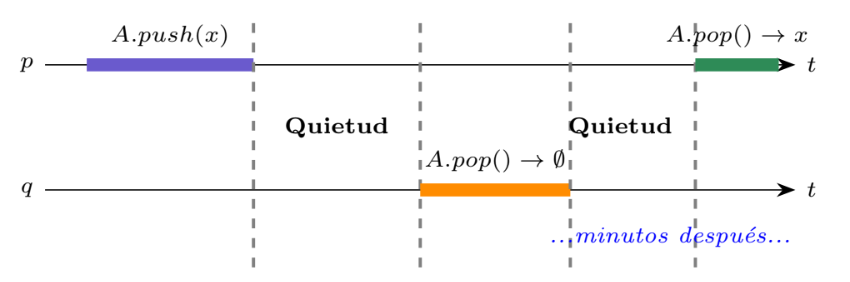
\includegraphics[width=0.8\textwidth]{Imagenes/image-4.png}
    \vspace{-10pt}
\end{figure}
\begin{enumerate}
    \item \textcolor{dkgreen}{¿Por qué esta ejecución cumple con Consistencia Eventual pero rompe la Consistencia en la Inactividad?}

    Esta ejecución cumple con \textbf{Consistencia Eventual} porque esta propiedad permite que se observen resultados atrasados, siempre y cuando eventualmente el sistema converja al estado correcto. Esto se cumple cuando $p$ realiza el $pop()$ y recibe $x$, ya que finalmente el sistema termina reflejando el estado final esperado.
    
    Por otro lado, no se cumple la \textbf{Consistencia en la Inactividad} porque entre el $push(x)$ y el $pop()$ de $q$ hubo un periodo de quietud. Por lo tanto, el $push(x)$ tuvo que haber quedado completamente antes del $pop()$ de $q$. En consecuencia, cuando $q$ realizó el $pop()$, la pila ya debía contener a $x$ y el resultado correcto era recibir $x$, pero recibió $null$. Como el periodo de quietud impide reordenar el $push(x)$ para colocarlo después del $pop()$, la ejecución no puede corresponder a un orden secuencial válido y se rompe la Consistencia en la Inactividad.
\end{enumerate}
